\exercise{Enhancement}
\subsection*{a - \texttt{IPlogenhance}}
Sometimes it can be desirable to increase the intensity of low-intensity pixels without affecting high-intensity pixels too much. A way to achieve this goal is by compressing the dynamic range of an image. By applying the log transform, an image may become more insightful than when the dynamic range is too large. The log transformation is: 
\[
  s = c\mbox{ }log(1+r)
\]
In this formula the value $r$ represents the value of the pixel the transformation is applied to. The value $c$ is a parameter chosen by the user. Implementing this formula is fairly straightforward in \textit{MATLAB} and we arrived at this solution directly by implementing the formula. The following \textit{MATLAB} code applies the log transformation to an image. 
\matlabexternal{IPlogenhance.m}
Here the type of \verb image  is a $y \times x$-matrix. The output image is a $y \times x$-matrix with the transformation applied.

\subsection*{b - Enhancing a fractured spine}
In order to make sure the implementation is correct and the log transformation is useful, the operation is applied to an image that could benefit from a compressed dynamic range.

Figure~\ref{fig:fractured_spine_original} shows an image of a fractured spine. Not all regions of interest are clearly visible; the image can benefit from some contrast enhancement.
Figure~\ref{fig:fractured_spines} shows images of a fractured spine were the value for \(c\) in the log transformation is varied.

It is clearly visible that the lowest values of \(c\) produce underexposed images, and the highest values of \(c\) produce overexposed images.
Both of these are not desirable, so the ideal value most be somewhere in between.

In our opinion, the values \(c=2\) and \(c=2.5\) produces the best results, since it looks like the best trade-off in enhancing areas that are darker while not overexposing values that already have higher brightness.
This is why we produced another set of images in that interval, which are shown in Figure~\ref{fig:fractured_spines_best}.

\begin{figure}[!Htb]
  \centering
  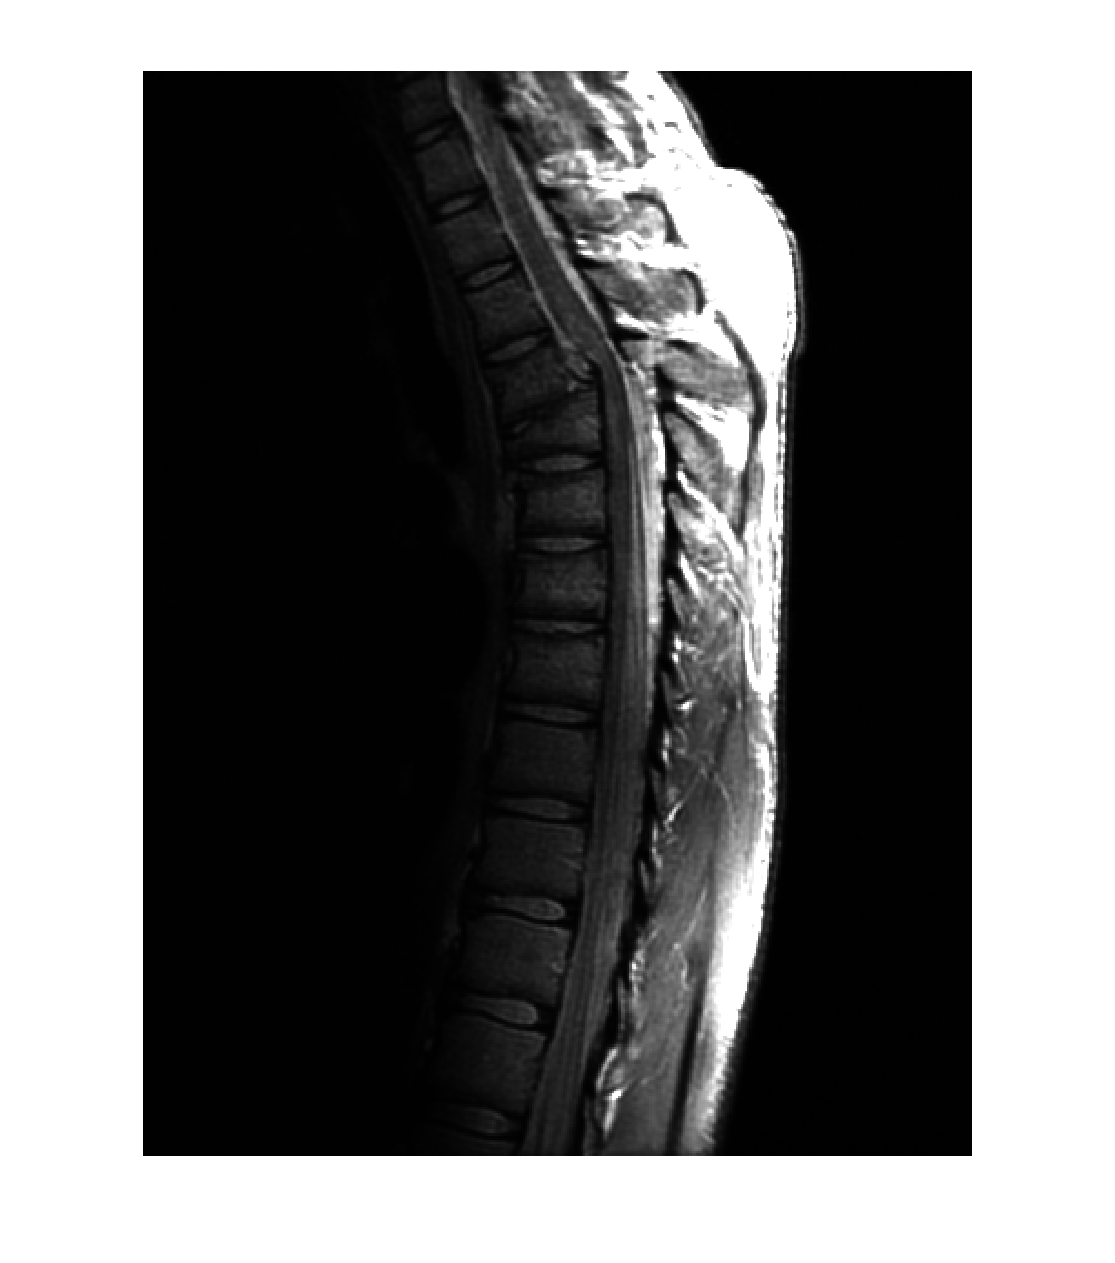
\includegraphics[width=\textwidth]{fracturedSpineOriginal.eps}
  \caption{Original fractured spine image.}
  \label{fig:fractured_spine_original}
\end{figure}

\begin{figure}[!Htb]
  \centering
  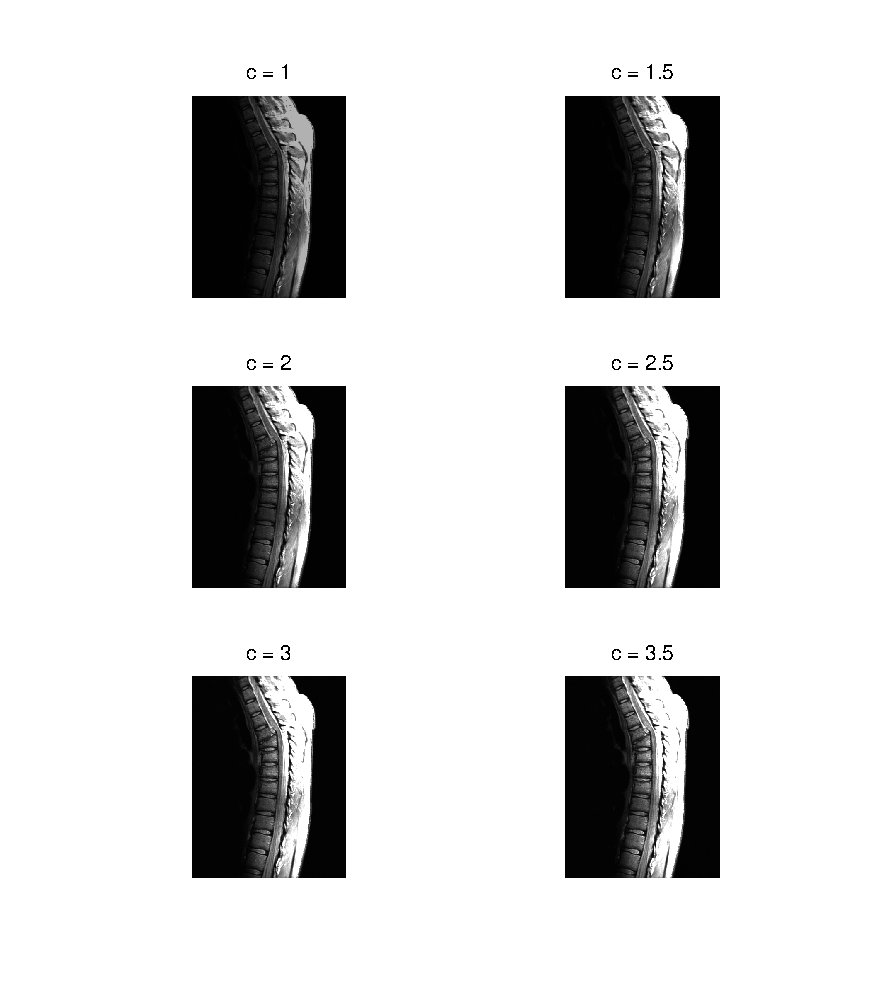
\includegraphics[width=\textwidth]{fracturedSpines.eps}
  \caption{Comparison of images of a fractured spine with different values for \(c\).}
  \label{fig:fractured_spines}
\end{figure}

\begin{figure}[!Htb]
  \centering
  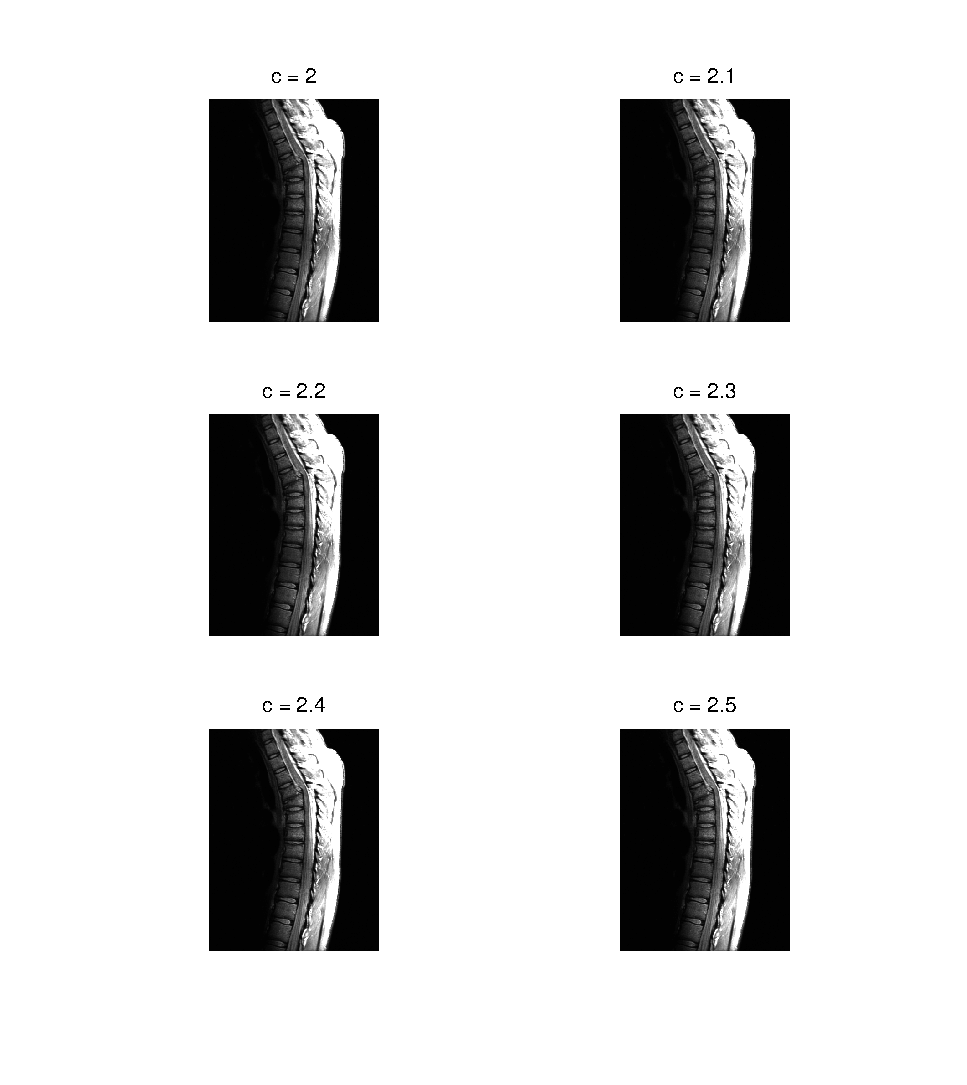
\includegraphics[width=\textwidth]{fracturedSpinesBest.eps}
  \caption{Comparison of images of a fractured spine with different values for \(c\). In our opinion, this interval shows the best results, since the contrast in the region of interest is enhanced. The image with \(c = 2.2\) is optimal, in our opinion.}
  \label{fig:fractured_spines_best}
\end{figure}

\clearpage